% ================================================================
% CPET Galois Ring Homomorphic Encryption — Presentation
% Compile: pdflatex presentation.tex (twice for TOC)
% ================================================================
\documentclass[aspectratio=169, 11pt]{beamer}

\usetheme{Madrid}
\usecolortheme{whale}
\setbeamertemplate{navigation symbols}{}
\setbeamertemplate{footline}[frame number]

\usepackage{amsmath, amssymb, mathtools}
\usepackage{booktabs}
\usepackage{tikz}
\usetikzlibrary{arrows.meta, positioning, shapes.geometric, fit, calc}
\usepackage{listings}
\usepackage{xcolor}

\definecolor{codegreen}{rgb}{0.0, 0.5, 0.0}
\definecolor{codegray}{rgb}{0.5, 0.5, 0.5}
\definecolor{codepurple}{rgb}{0.58, 0, 0.82}
\definecolor{backcolour}{rgb}{0.95, 0.95, 0.97}

\lstset{
  backgroundcolor=\color{backcolour},
  basicstyle=\ttfamily\tiny,
  keywordstyle=\color{blue}\bfseries,
  commentstyle=\color{codegreen},
  stringstyle=\color{codepurple},
  breaklines=true,
  frame=single,
  columns=fullflexible,
}

\title{CPET Galois Ring Package}
\subtitle{Homomorphic Encryption with Hardware-Accelerated Verification}
\author{Presenter Name}
\date{\today}

% ================================================================
\begin{document}

% ------ TITLE ------
\begin{frame}
\titlepage
\end{frame}

% ------ OUTLINE ------
\begin{frame}{Outline}
\tableofcontents
\end{frame}

% ================================================================
\section{Overview}
% ================================================================

\begin{frame}{Project Overview}
\begin{itemize}
    \item \textbf{Goal:} Compute on encrypted data without decryption
    \item \textbf{Scheme:} BV (Brakerski--Vaikuntanathan) homomorphic encryption
    \item \textbf{Ring:} Polynomials in $\mathbb{Z}_q[X]/(X^N+1)$, \; $N = 2^{13} = 8192$
    \item \textbf{Implementation:} Pure Python 3.12 (no external dependencies)
    \item \textbf{Hardware:} Optional Verilog acceleration via Verilator
\end{itemize}

\vspace{0.5em}
\begin{block}{Key Features}
\begin{enumerate}
    \item Full HE pipeline: \texttt{Encode $\to$ Encrypt $\to$ Evaluate $\to$ Decrypt}
    \item Residue Number System (RNS) for large modulus arithmetic
    \item Number Theoretic Transform (NTT) for fast polynomial multiplication
    \item Homomorphic hash verification (SW + HW backends)
    \item Arithmetic circuit parser and evaluator
\end{enumerate}
\end{block}
\end{frame}

% ================================================================
\section{Mathematical Foundations}
% ================================================================

\begin{frame}{Polynomial Ring}
All operations live in the \textbf{negacyclic polynomial ring}:
\[
    R_q \;=\; \mathbb{Z}_q[X]\big/\!\left(X^N + 1\right), \qquad N = 2^{13},\quad q \text{ prime}
\]

\begin{itemize}
    \item Elements are polynomials of degree $< N$ with coefficients in $(-q/2,\; q/2]$
    \item \textbf{Negacyclic property:} $X^N \equiv -1$, so $X^{N+k} \equiv -X^k$
    \item Coefficient representation: \textbf{centered modular reduction}
\end{itemize}

\vspace{0.5em}
\begin{block}{Example}
Let $N=4$, $q=17$. If $a(X) = 1 + 2X + 3X^2$ and $b(X) = 4X^2 + 5X^3$, then
\[
    a \cdot b = 4X^4 + \cdots \;\equiv\; -4 + \cdots \pmod{X^4+1,\; 17}
\]
\end{block}
\end{frame}

\begin{frame}{Residue Number System (RNS)}
\textbf{Problem:} Modulus $Q = \prod p_i$ can be 100+ bits.

\textbf{Solution:} Decompose into small independent lanes.

\vspace{0.5em}
\begin{columns}[T]
\column{0.48\textwidth}
\textbf{Decomposition:}
\[
    c \;\longrightarrow\; \bigl(c \bmod p_1,\; c \bmod p_2,\; c \bmod p_3\bigr)
\]
\begin{itemize}
    \item Each $p_i$ is 30--40 bits
    \item Arithmetic per lane is independent
    \item Fully parallelizable
\end{itemize}

\column{0.48\textwidth}
\textbf{Recovery (CRT):}
\[
    c = \sum_{i} r_i \cdot M_i \cdot y_i \bmod Q
\]
where $M_i = Q/p_i$ and $y_i \equiv M_i^{-1} \pmod{p_i}$

\vspace{0.5em}
\textbf{Input:} Residues $(r_1, r_2, r_3)$\\
\textbf{Output:} Original $c \in \mathbb{Z}_Q$
\end{columns}

\vspace{0.5em}
\begin{block}{Data Structure}
\texttt{RNS\_Poly} = \texttt{dict[prime $\to$ Poly]} \;---\; one polynomial per prime lane
\end{block}
\end{frame}

\begin{frame}{Number Theoretic Transform (NTT)}
\textbf{Problem:} Polynomial multiplication is $O(N^2)$ (schoolbook).

\textbf{Solution:} NTT reduces to $O(N \log N)$ via pointwise multiply.

\vspace{0.5em}
\begin{center}
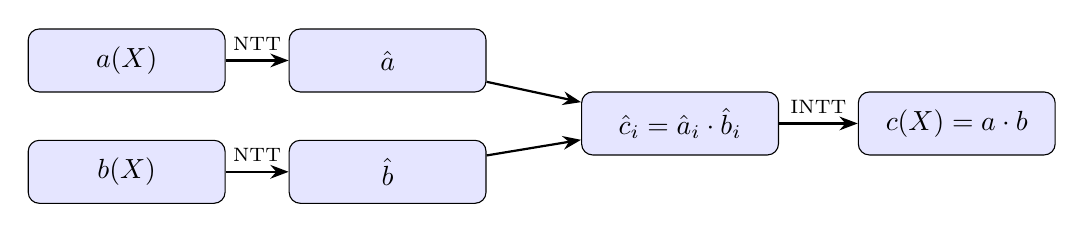
\begin{tikzpicture}[
    box/.style={draw, rounded corners, minimum width=2.5cm, minimum height=0.8cm, fill=blue!10},
    arr/.style={-{Stealth}, thick}
]
\node[box] (a) {$a(X)$};
\node[box, right=0.8cm of a] (antt) {$\hat{a}$};
\node[box, below=0.6cm of a] (b) {$b(X)$};
\node[box, right=0.8cm of b] (bntt) {$\hat{b}$};
\node[box, right=1.2cm of antt, yshift=-0.8cm] (cntt) {$\hat{c}_i = \hat{a}_i \cdot \hat{b}_i$};
\node[box, right=1.0cm of cntt] (c) {$c(X) = a \cdot b$};

\draw[arr] (a) -- node[above]{\scriptsize NTT} (antt);
\draw[arr] (b) -- node[above]{\scriptsize NTT} (bntt);
\draw[arr] (antt) -- (cntt);
\draw[arr] (bntt) -- (cntt);
\draw[arr] (cntt) -- node[above]{\scriptsize INTT} (c);
\end{tikzpicture}
\end{center}

\begin{columns}[T]
\column{0.48\textwidth}
\textbf{Forward (Cooley--Tukey):}
\begin{itemize}
    \item Normal order $\to$ Bit-reversed
    \item Butterfly: $u' = u + vw$, \; $v' = u - vw$
\end{itemize}

\column{0.48\textwidth}
\textbf{Inverse (Gentleman--Sande):}
\begin{itemize}
    \item Bit-reversed $\to$ Normal order
    \item Butterfly: $u' = u + v$, \; $v' = (u-v)w$
    \item Final scaling: $\times N^{-1}$
\end{itemize}
\end{columns}

\vspace{0.3em}
\textbf{Requirement:} NTT-friendly primes $p \equiv 1 \pmod{2N}$
\end{frame}

% ================================================================
\section{HE Pipeline}
% ================================================================

\begin{frame}{Full Pipeline Overview}
\begin{center}
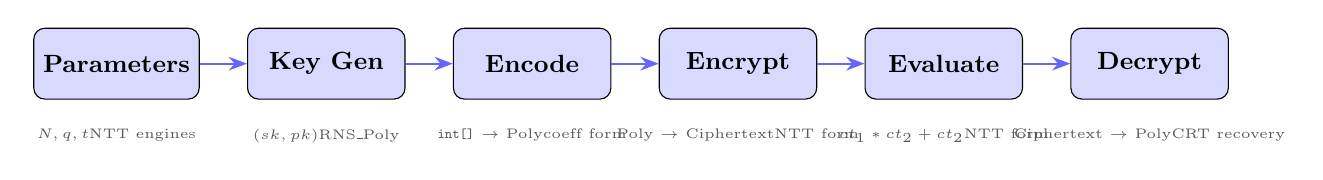
\begin{tikzpicture}[
    stage/.style={draw, rounded corners, minimum width=2.0cm, minimum height=0.9cm,
                  fill=blue!15, font=\small\bfseries, align=center},
    data/.style={font=\tiny, text=gray!70!black},
    arr/.style={-{Stealth}, thick, color=blue!60},
    node distance=0.5cm and 0.5cm
]
\node[stage] (param) {Parameters};
\node[stage, right=0.6cm of param] (keygen) {Key Gen};
\node[stage, right=0.6cm of keygen] (encode) {Encode};
\node[stage, right=0.6cm of encode] (encrypt) {Encrypt};
\node[stage, right=0.6cm of encrypt] (eval) {Evaluate};
\node[stage, right=0.6cm of eval] (decrypt) {Decrypt};

\draw[arr] (param) -- (keygen);
\draw[arr] (keygen) -- (encode);
\draw[arr] (encode) -- (encrypt);
\draw[arr] (encrypt) -- (eval);
\draw[arr] (eval) -- (decrypt);

% Inputs/Outputs below
\node[data, below=0.25cm of param] {$N, q, t$\\NTT engines};
\node[data, below=0.25cm of keygen] {$(sk, pk)$\\RNS\_Poly};
\node[data, below=0.25cm of encode] {\texttt{int[]} $\to$ Poly\\coeff form};
\node[data, below=0.25cm of encrypt] {Poly $\to$ Ciphertext\\NTT form};
\node[data, below=0.25cm of eval] {$ct_1 \ast ct_2 + ct_2$\\NTT form};
\node[data, below=0.25cm of decrypt] {Ciphertext $\to$ Poly\\CRT recovery};
\end{tikzpicture}
\end{center}
\end{frame}

\begin{frame}{Stage 1: Parameter Setup}
\textbf{Input:} Scheme type, polynomial degree, modulus sizes, plaintext modulus, bounds

\vspace{0.3em}
\begin{center}
\begin{tabular}{lll}
\toprule
\textbf{Parameter} & \textbf{Value} & \textbf{Purpose} \\
\midrule
\texttt{scheme} & \texttt{"bv"} & BV homomorphic encryption \\
\texttt{poly\_modulus} & $2^{13} = 8192$ & Ring degree $N$ \\
\texttt{coeff\_modulus} & $[30, 30, 40]$ bits & RNS prime sizes \\
\texttt{plain\_modulus} & $18$ bits & Plaintext space modulus $t$ \\
\texttt{bound} & $(1, 2)$ & Secret key bound, error bound \\
\bottomrule
\end{tabular}
\end{center}

\vspace{0.3em}
\textbf{Output:}
\begin{itemize}
    \item NTT-friendly primes $p_i \equiv 1 \pmod{2N}$ for each RNS lane
    \item NTT engine per prime (precomputed twiddle tables $\psi^{\text{bit\_rev}(i)}$)
    \item CRT basis weights $M_i \cdot y_i$ for reconstruction
    \item Total modulus $Q = \prod p_i$
\end{itemize}
\end{frame}

\begin{frame}{Stage 2: Key Generation}
\textbf{Input:} \texttt{HE\_Parameter} context

\vspace{0.5em}
\begin{columns}[T]
\column{0.48\textwidth}
\textbf{Secret Key $sk$:}
\begin{enumerate}
    \item Sample random polynomial
    \item Coefficients $\in [-1, +1]$ (ternary)
    \item Decompose into RNS lanes
    \item Transform to NTT form
\end{enumerate}
\textbf{Output:} \texttt{RNS\_Poly} (NTT form)

\vspace{0.3em}
\textbf{Precomputation:}
\[
    sk^1, sk^2, \ldots, sk^{40}
\]
Needed for decrypting multi-component ciphertexts.

\column{0.48\textwidth}
\textbf{Public Key $pk = (c_0, c_1)$:}
\begin{enumerate}
    \item $c_0 \gets$ random \texttt{RNS\_Poly}
    \item $c_1 = c_0 \times sk$
    \item $pk = \texttt{Ciphertext}([c_0, -c_1])$
\end{enumerate}
\textbf{Output:} \texttt{Ciphertext} of size 2, NTT form

\vspace{0.3em}
\textbf{Invariant:}
\[
    c_0 + c_1 \cdot sk = c_0 - c_0 \cdot sk \cdot sk \approx 0
\]
\end{columns}
\end{frame}

\begin{frame}{Stage 3: Encoding}
\textbf{Input:} Integer list $[m_0, m_1, \ldots]$

\textbf{Output:} \texttt{Poly} in coefficient form, modulus $= t$ (plain modulus)

\vspace{0.5em}
\begin{columns}[T]
\column{0.48\textwidth}
\textbf{Coefficient Encoding:}
\[
    [1, 2, 3] \;\longrightarrow\; 1 + 2X + 3X^2
\]
\begin{itemize}
    \item Direct mapping: integer $\to$ coefficient
    \item Padded with zeros to degree $N-1$
    \item Stays in \textbf{coefficient form} (not NTT)
\end{itemize}

\column{0.48\textwidth}
\textbf{Slot Encoding:}
\[
    [v_0, v_1, \ldots] \;\longrightarrow\; \text{Poly}
\]
\begin{itemize}
    \item SIMD-like packing
    \item Each ``slot'' holds independent value
    \item Enables parallel computation
\end{itemize}
\end{columns}
\end{frame}

\begin{frame}{Stage 4: Encryption}
\textbf{Input:} Public key $pk$, plaintext polynomial $m(X)$

\vspace{0.3em}
\textbf{Process:}
\[
    \text{ct} = pk.\text{copy}() \;;\quad \text{ct}[-1] \mathrel{+}= m
\]
\[
    \text{ct} = \bigl[\,c_0,\;\; {-c_1 + m}\,\bigr]
\]

\vspace{0.3em}
\textbf{Output:} \texttt{Ciphertext} of size 2, NTT form

\vspace{0.5em}
\begin{block}{Decryption Correctness}
\[
    c_0 + c_1 \cdot sk = c_0 + (-c_0 \cdot sk + m) \cdot sk = m + \text{noise}
\]
Decryption works as long as $|\text{noise}| < t/2$.
\end{block}

\vspace{0.3em}
\textbf{Initial error bound:} $e_0 = 2$
\end{frame}

\begin{frame}{Stage 5: Homomorphic Evaluation}
\textbf{Ciphertext Addition:} $\text{ct}_3 = \text{ct}_1 + \text{ct}_2$
\[
    \text{ct}_3[i] = \text{ct}_1[i] + \text{ct}_2[i] \quad \forall\, i
    \qquad\qquad
    e_3 = e_1 + e_2
\]

\vspace{0.3em}
\textbf{Ciphertext Multiplication:} $\text{ct}_3 = \text{ct}_1 \times \text{ct}_2$
\[
    \text{ct}_3[k] = \sum_{i+j=k} \text{ct}_1[i] \cdot \text{ct}_2[j]
    \qquad\qquad
    e_3 = e_1 \cdot e_2 + (e_1 + e_2)\cdot t
\]

\vspace{0.3em}
\begin{center}
\begin{tabular}{lccc}
\toprule
\textbf{Operation} & \textbf{Output Size} & \textbf{Error Growth} & \textbf{Form} \\
\midrule
Addition & $\max(|ct_1|, |ct_2|)$ & $e_1 + e_2$ & NTT \\
Multiplication & $|ct_1| + |ct_2| - 1$ & $e_1 e_2 + (e_1+e_2)t$ & NTT \\
Plain multiply & $|ct|$ & $e \cdot \|m\|_\infty$ & NTT \\
\bottomrule
\end{tabular}
\end{center}

\vspace{0.3em}
\textbf{Depth limit:} Noise grows exponentially $\Rightarrow$ bounded multiplicative depth.
\end{frame}

\begin{frame}{Stage 6: Decryption}
\textbf{Input:} Ciphertext $\text{ct} = [c_0, c_1, \ldots, c_{k-1}]$, secret key $sk$

\vspace{0.5em}
\textbf{Step 1 --- Polynomial evaluation (NTT form):}
\[
    \text{result} = \sum_{i=0}^{k-1} c_i \cdot sk^{i}
\]
Each $c_i \cdot sk^i$ is a pointwise multiplication in NTT domain.

\vspace{0.3em}
\textbf{Step 2 --- Inverse NTT:}
\[
    \text{result} \xleftarrow{\text{INTT}} \text{coefficient form}
\]

\textbf{Step 3 --- CRT Recovery:}
\[
    \text{For each coefficient:} \quad
    m_j = \biggl(\sum_{i} r_{i,j} \cdot M_i \cdot y_i \bmod Q\biggr) \bmod t
\]

\vspace{0.3em}
\textbf{Output:} Plaintext \texttt{Poly} in coefficient form, modulus $= t$
\end{frame}

% ================================================================
\section{Proof and Verification}
% ================================================================

\begin{frame}{Homomorphic Hash --- Cipher Hash}
\textbf{Goal:} Fingerprint a ciphertext that respects homomorphic operations.

\vspace{0.3em}
\textbf{Squaring-power Horner evaluation:}
\[
    H(\text{ct}, r) = \text{ct}[0] \cdot r^{2^{k-1}} + \text{ct}[1] \cdot r^{2^{k-2}} + \cdots + \text{ct}[k-2] \cdot r + \text{ct}[k-1]
\]

\textbf{Algorithm:}
\begin{enumerate}
    \item $\text{acc} \gets \text{ct}[\text{last}]$
    \item $r_{\text{pow}} \gets r$
    \item For $i$ from $\text{last}-1$ down to $0$:
    \begin{itemize}
        \item $\text{acc} \mathrel{+}= \text{ct}[i] \times r_{\text{pow}}$
        \item $r_{\text{pow}} \gets r_{\text{pow}} \times r_{\text{pow}}$ \quad (squaring)
    \end{itemize}
\end{enumerate}

\vspace{0.3em}
\textbf{Input:} Ciphertext (list of RNS\_Poly), random polynomial $r$

\textbf{Output:} Single \texttt{RNS\_Poly} (the hash fingerprint)

\vspace{0.3em}
\begin{block}{Homomorphic Property}
\[
    H(ct_1 \times ct_2) = H(ct_1) \times H(ct_2), \qquad
    H(ct_1 + ct_2) = H(ct_1) + H(ct_2)
\]
\end{block}
\end{frame}

\begin{frame}{Hash Verification}
\textbf{Verify:} $\text{ct}_3 = \text{ct}_1 \times \text{ct}_2 + \text{ct}_2$ \quad \textbf{without decryption!}

\vspace{0.5em}
\textbf{Protocol:}
\begin{enumerate}
    \item Compute $h_1 = H(\text{ct}_1, r)$
    \item Compute $h_2 = H(\text{ct}_2, r)$
    \item Compute $h_3 = H(\text{ct}_3, r)$
    \item Compute $\text{expected} = h_1 \times h_2 + h_2$
    \item \textbf{Check:} $h_3 \stackrel{?}{=} \text{expected}$
\end{enumerate}

\vspace{0.5em}
\begin{center}
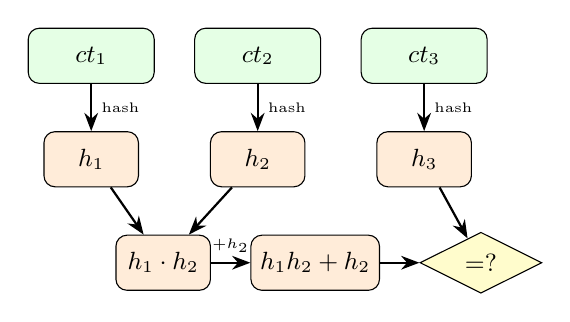
\begin{tikzpicture}[
    box/.style={draw, rounded corners, minimum width=1.6cm, minimum height=0.7cm, fill=green!10, font=\small},
    res/.style={draw, rounded corners, minimum width=1.2cm, minimum height=0.7cm, fill=orange!15, font=\small},
    arr/.style={-{Stealth}, thick}
]
\node[box] (c1) {$ct_1$};
\node[box, right=0.5cm of c1] (c2) {$ct_2$};
\node[box, right=0.5cm of c2] (c3) {$ct_3$};

\node[res, below=0.6cm of c1] (h1) {$h_1$};
\node[res, below=0.6cm of c2] (h2) {$h_2$};
\node[res, below=0.6cm of c3] (h3) {$h_3$};

\draw[arr] (c1) -- node[right, font=\tiny]{hash} (h1);
\draw[arr] (c2) -- node[right, font=\tiny]{hash} (h2);
\draw[arr] (c3) -- node[right, font=\tiny]{hash} (h3);

\node[res, below right=0.6cm and -0.3cm of h1] (mul) {$h_1 \cdot h_2$};
\node[res, right=0.5cm of mul] (exp) {$h_1 h_2 + h_2$};

\draw[arr] (h1) -- (mul);
\draw[arr] (h2) -- (mul);
\draw[arr] (mul) -- node[above, font=\tiny]{$+h_2$} (exp);

\node[draw, diamond, aspect=2, right=0.5cm of exp, fill=yellow!20, font=\small] (cmp) {$=$?};
\draw[arr] (exp) -- (cmp);
\draw[arr] (h3) -- (cmp);
\end{tikzpicture}
\end{center}
\end{frame}

\begin{frame}{Arithmetic Circuit Evaluation}
\textbf{Input:} Expression string, e.g.\ \texttt{"0*1+2"}

\textbf{Output:} Leveled \texttt{Circuit} of \texttt{Gate}s (ADD / MULT)

\vspace{0.5em}
\textbf{Parse pipeline:}
\begin{enumerate}
    \item \textbf{Tokenize:} \texttt{"0*1+2"} $\to$ \texttt{[0, *, 1, +, 2]}
    \item \textbf{Shunting-yard:} Infix $\to$ Postfix: \texttt{[0, 1, *, 2, +]}
    \item \textbf{Build DAG:} Tree of operation nodes with depth tracking
    \item \textbf{Balance:} Min-heap (Huffman-style) to minimize circuit depth
    \item \textbf{Levelize:} Convert to layer-by-layer gates with pass-through wires
    \item \textbf{Pad:} Each layer padded to power-of-2 gate count
\end{enumerate}

\vspace{0.3em}
\textbf{Supported computations on gates:}

\begin{center}
\begin{tabular}{ll}
\toprule
\textbf{Method} & \textbf{Operand Types} \\
\midrule
\texttt{compute\_poly} & Poly, RNS\_Poly, Ciphertext \\
\texttt{compute\_int}  & Integers (mod $q$) \\
\texttt{compute\_field} & Field elements \\
\bottomrule
\end{tabular}
\end{center}
\end{frame}

% ================================================================
\section{Hardware Acceleration}
% ================================================================

\begin{frame}{What Was Moved to Hardware (and What Was Not)}
\textbf{Principle:} Only the \emph{compute engines} are ported --- not the data-organization layers.

\vspace{0.5em}
\begin{center}
\small
\begin{tabular}{@{}lll@{}}
\toprule
\textbf{Component} & \textbf{In hardware?} & \textbf{Why} \\
\midrule
NTT / INTT engine & \textbf{Yes} (\texttt{ntt\_hw.so}) & Core kernel --- used by every operation \\
Hash + verify & \textbf{Yes} (\texttt{hash\_verifier\_hw.so}) & Fingerprint + check fused in one circuit \\
\midrule
\texttt{RNS\_Poly} & No & A \emph{concept}, not an engine --- pure dispatch \\
\texttt{Ciphertext} / \texttt{Encryptor} / \dots & No & Orchestration; calls the engines \\
CRT recovery & No & Runs once at decrypt, off the hot path \\
\bottomrule
\end{tabular}
\end{center}

\vspace{0.5em}
\begin{block}{Why no ``RNS hardware''?}
\texttt{RNS\_Poly} owns no arithmetic --- every op just loops over primes and delegates to
the per-lane \texttt{Poly}, which calls the NTT engine. Hardening one prime's NTT
automatically accelerates the whole RNS system: \emph{RNS = run the engine once per prime}.
\end{block}
\end{frame}

\begin{frame}{Verilog Module Hierarchy}
\begin{center}
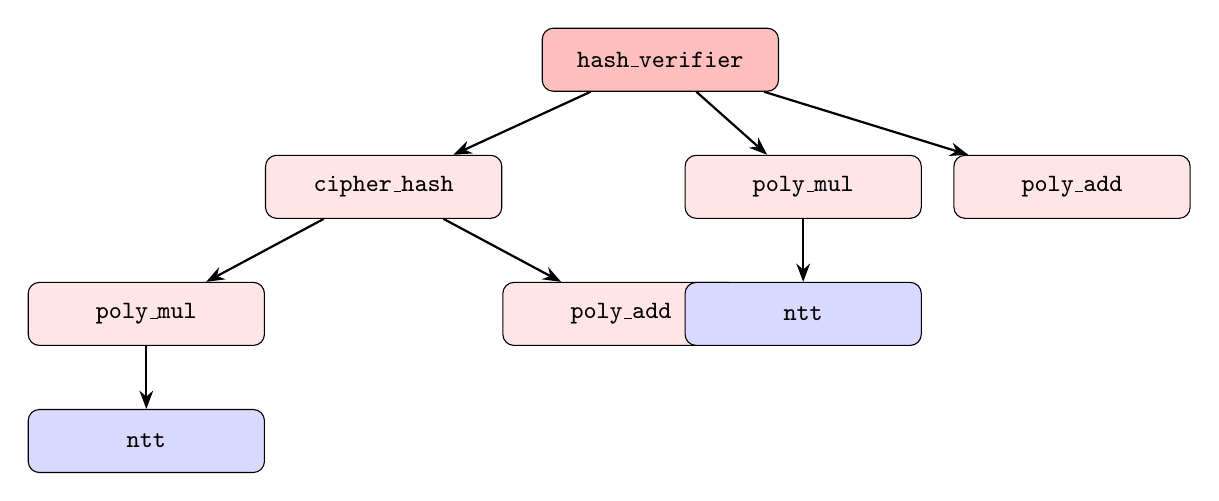
\begin{tikzpicture}[
    mod/.style={draw, rounded corners, minimum width=3.0cm, minimum height=0.8cm, fill=red!10, font=\small\ttfamily},
    arr/.style={-{Stealth}, thick},
    node distance=0.4cm
]
\node[mod, fill=red!25] (hv) {hash\_verifier};

\node[mod, below left=0.8cm and 0.5cm of hv] (ch) {cipher\_hash};
\node[mod, below right=0.8cm and -1.2cm of hv] (pm2) {poly\_mul};
\node[mod, right=0.4cm of pm2] (pa2) {poly\_add};

\node[mod, below left=0.8cm and 0.0cm of ch] (pm1) {poly\_mul};
\node[mod, below right=0.8cm and 0.0cm of ch] (pa1) {poly\_add};

\node[mod, below=0.8cm of pm1, fill=blue!15] (ntt1) {ntt};
\node[mod, below=0.8cm of pm2, fill=blue!15] (ntt2) {ntt};

\draw[arr] (hv) -- (ch);
\draw[arr] (hv) -- (pm2);
\draw[arr] (hv) -- (pa2);
\draw[arr] (ch) -- (pm1);
\draw[arr] (ch) -- (pa1);
\draw[arr] (pm1) -- (ntt1);
\draw[arr] (pm2) -- (ntt2);
\end{tikzpicture}
\end{center}

\vspace{0.3em}
\begin{center}
\small
\begin{tabular}{lll}
\toprule
\textbf{Module} & \textbf{Function} & \textbf{Params} \\
\midrule
\texttt{ntt} & Cooley--Tukey / Gentleman--Sande, Barrett reduction & LOGN=13, Q\_WIDTH=40 \\
\texttt{poly\_add} & $(a[i] \pm b[i]) \bmod q$, one coeff/cycle & LOGN=13, Q\_WIDTH=40 \\
\texttt{poly\_mul} & NTT(a) $\to$ NTT(b) $\to$ pointwise $\to$ INTT & shared NTT unit \\
\texttt{cipher\_hash} & Horner hash with squaring powers of $r$ & CT\_SIZE=3 \\
\texttt{hash\_verifier} & $H(c_3) \stackrel{?}{=} H(c_1)H(c_2) + H(c_2)$ & top level \\
\bottomrule
\end{tabular}
\end{center}
\end{frame}

\begin{frame}{NTT Hardware Engine}
\textbf{Architecture:} One butterfly per 2-clock micro-cycle (READ $\to$ WRITE)

\vspace{0.3em}
\textbf{FSM:}
\begin{center}
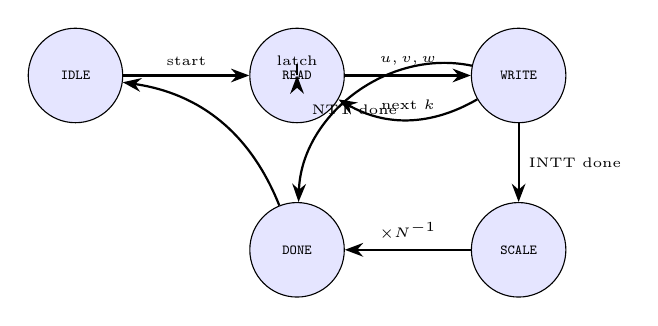
\begin{tikzpicture}[
    state/.style={draw, circle, minimum size=1.2cm, font=\tiny\ttfamily, fill=blue!10},
    arr/.style={-{Stealth}, thick, font=\tiny},
    node distance=1.6cm
]
\node[state] (idle) {IDLE};
\node[state, right=of idle] (read) {READ};
\node[state, right=of read] (write) {WRITE};
\node[state, below=1.0cm of write] (scale) {SCALE};
\node[state, left=of scale] (done) {DONE};

\draw[arr] (idle) -- node[above]{start} (read);
\draw[arr] (read) -- node[above]{latch} (read);
\draw[arr] (read) -- node[above]{$u,v,w$} (write);
\draw[arr] (write) to[bend left=30] node[above]{next $k$} (read);
\draw[arr] (write) -- node[right]{INTT done} (scale);
\draw[arr] (write) to[bend right=50] node[below]{NTT done} (done);
\draw[arr] (scale) -- node[above]{$\times N^{-1}$} (done);
\draw[arr] (done) to[bend right=30] (idle);
\end{tikzpicture}
\end{center}

\vspace{0.3em}
\textbf{Key design:}
\begin{itemize}
    \item Barrett reduction for modular multiply (synthesizable, no \texttt{\%})
    \item Runtime-configurable $q$, $N^{-1}$, Barrett constant $M$
    \item Twiddle tables loaded via write port (forward + inverse)
\end{itemize}
\end{frame}

\begin{frame}{NTT Engine Parameters}
\textbf{Compile-time parameters} (Verilog \texttt{parameter}, set in \texttt{Makefile}):
\begin{center}
\small
\begin{tabular}{@{}llll@{}}
\toprule
\textbf{Param} & \textbf{Default} & \textbf{Meaning} & \textbf{Derived} \\
\midrule
\texttt{LOGN}    & 13 & $\log_2 N$ & $N = 1\!\ll\!\texttt{LOGN} = 8192$ \\
\texttt{Q\_WIDTH} & 40 & modulus/coeff bit-width & \texttt{BARRETT\_K} $= 2\,Q_W = 80$ \\
\texttt{CT\_SIZE} & 3 & max ciphertext components & --- \\
\bottomrule
\end{tabular}
\end{center}
\hspace{1em}\scriptsize Also derived: \texttt{K\_MAX}$=N/2-1$ (butterflies/stage), \texttt{S\_MAX}$=$\texttt{LOGN}$-1$ (stages).

\vspace{0.5em}
\normalsize
\textbf{Runtime inputs} (loaded per RNS prime, so one core serves all lanes):
\begin{center}
\small
\begin{tabular}{@{}lll@{}}
\toprule
\textbf{Input} & \textbf{Width} & \textbf{Meaning} \\
\midrule
\texttt{q}         & \texttt{Q\_WIDTH} & NTT-friendly prime, $q \equiv 1 \pmod{2N}$ \\
\texttt{n\_inv}    & \texttt{Q\_WIDTH} & $N^{-1} \bmod q$ --- final INTT scaling \\
\texttt{barrett\_m} & $2\cdot$\texttt{Q\_WIDTH} & $\lfloor 2^{2 Q_W}/q \rfloor$ --- Barrett reduction constant \\
\texttt{inverse}   & 1 bit & $0 = $ NTT, \; $1 = $ INTT \\
\texttt{tw[\,]}      & $2N \times$\texttt{Q\_WIDTH} & twiddle ROM: fwd $[0,N)$, inv $[N,2N)$ \\
\bottomrule
\end{tabular}
\end{center}
\textbf{Why runtime?} Keeping $q$, $N^{-1}$, $M$ as inputs lets \emph{one} compiled core handle every RNS prime.
\end{frame}

\begin{frame}{Inside the Hardware: Storage \& Reuse}
\textbf{Ciphertext store --- where the cipher is loaded:}
\begin{itemize}
    \item Streamed in from live \texttt{Ciphertext} objects (per RNS prime), \emph{not} from files
    \item Path: \texttt{c\{1,2,3\}.\_data} $\to$ ctypes \texttt{hv\_load\_ct} $\to$ write ports
    \item Lands in a 3-D memory: \quad
          \texttt{ct\_mem[ct\_id][ct\_sel][addr]} \quad (\texttt{ct\_id}: 0=$c_1$,1=$c_2$,2=$c_3$)
\end{itemize}

\vspace{0.4em}
\textbf{Twiddle factors --- one shared ROM in \texttt{ntt.v}:}
\[
    \texttt{reg [Q\_WIDTH-1:0] tw [0:2N-1]} \qquad
    \underbrace{[0,\,N)}_{\text{forward}} \;\;
    \underbrace{[N,\,2N)}_{\text{inverse}}
\]
\begin{itemize}
    \item Loaded once via \texttt{tw\_wr\_*}; \texttt{cipher\_hash} / \texttt{hash\_verifier} just forward the port down
    \item Inverse transform selects upper half by an $N$-offset on the read index
\end{itemize}

\vspace{0.4em}
\textbf{One hasher, reused three times (no duplicate hashing):}
\begin{itemize}
    \item \texttt{hash\_verifier} instantiates a \emph{single} \texttt{cipher\_hash} unit
    \item FSM drives it 3$\times$: \texttt{HASH\_C1}$\to h_1$, \texttt{HASH\_C2}$\to h_2$, \texttt{HASH\_C3}$\to h_3$
    \item Final compare reuses the \texttt{poly\_mul}/\texttt{poly\_add} already inside \texttt{cipher\_hash}
\end{itemize}
\end{frame}

\begin{frame}{SW/HW Integration}
\begin{center}
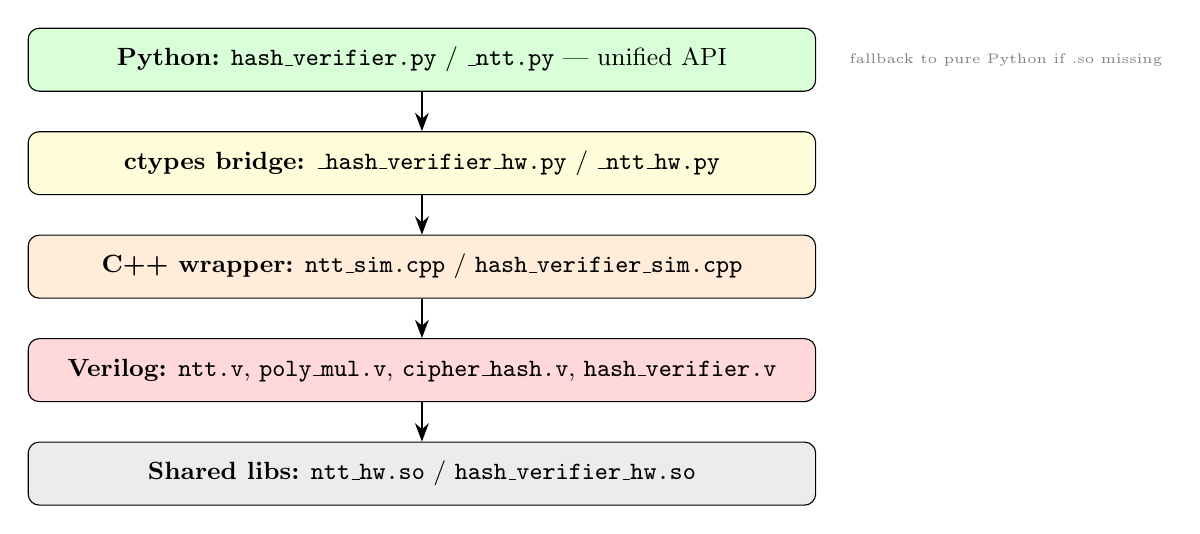
\begin{tikzpicture}[
    layer/.style={draw, rounded corners, minimum width=10cm, minimum height=0.8cm, font=\small},
    arr/.style={-{Stealth}, thick},
    node distance=0.5cm
]
\node[layer, fill=green!15] (py) {\textbf{Python:} \texttt{hash\_verifier.py} / \texttt{\_ntt.py} --- unified API};
\node[layer, fill=yellow!15, below=of py] (ct) {\textbf{ctypes bridge:} \texttt{\_hash\_verifier\_hw.py} / \texttt{\_ntt\_hw.py}};
\node[layer, fill=orange!15, below=of ct] (cpp) {\textbf{C++ wrapper:} \texttt{ntt\_sim.cpp} / \texttt{hash\_verifier\_sim.cpp}};
\node[layer, fill=red!15, below=of cpp] (ver) {\textbf{Verilog:} \texttt{ntt.v}, \texttt{poly\_mul.v}, \texttt{cipher\_hash.v}, \texttt{hash\_verifier.v}};
\node[layer, fill=gray!15, below=of ver] (so) {\textbf{Shared libs:} \texttt{ntt\_hw.so} / \texttt{hash\_verifier\_hw.so}};

\draw[arr] (py) -- (ct);
\draw[arr] (ct) -- (cpp);
\draw[arr] (cpp) -- (ver);
\draw[arr] (ver) -- (so);

\node[right=0.3cm of py, font=\tiny, text=gray] {fallback to pure Python if .so missing};
\end{tikzpicture}
\end{center}

\vspace{0.3em}
\textbf{Build:} \texttt{cd verilog/ \&\& make} $\to$ \texttt{ntt\_hw.so}\\
\texttt{make hash\_verifier} $\to$ \texttt{hash\_verifier\_hw.so}

\vspace{0.3em}
\textbf{Graceful fallback:} If \texttt{.so} not found, Python backend used automatically.
\end{frame}

\begin{frame}{Test Vector Cross-Validation}
\textbf{Strategy:} compute in software, feed the \emph{same} data to hardware, check the responses match (bit-exact).

\vspace{0.3em}
\begin{center}
\scriptsize
\texttt{gen\_test\_vectors.py} (SW engine) $\to$ \texttt{tv\_*.hex}
$\xrightarrow{\;\$readmemh\;}$ Verilog DUT recomputes
$\xrightarrow{\;===\;}$ match vs.\ \texttt{tv\_h*} (else \texttt{\$error})
\end{center}

\vspace{0.3em}
Inputs ($c_1,c_2,c_3,r$, twiddles, params) drive the DUT; \texttt{tv\_h1/h2/h3.hex} are the \emph{answer key}.
The live ctypes path does the same comparison straight from in-memory ciphertexts (no files).

\vspace{0.5em}
\begin{columns}[T]
\column{0.45\textwidth}
\textbf{Inputs (from Python):}
\begin{itemize}
    \item \texttt{tv\_params.hex} --- $q, N^{-1}$, Barrett $M$
    \item \texttt{tv\_twiddles\_fwd.hex} --- $\psi^{\text{br}(i)} \bmod q$
    \item \texttt{tv\_twiddles\_inv.hex} --- $\psi^{-\text{br}(i)} \bmod q$
    \item \texttt{tv\_r.hex} --- random polynomial $r$
    \item \texttt{tv\_c1\_*.hex} --- ciphertext $c_1$ components
    \item \texttt{tv\_c2\_*.hex} --- ciphertext $c_2$ components
    \item \texttt{tv\_c3\_*.hex} --- ciphertext $c_3$ components
\end{itemize}

\column{0.45\textwidth}
\textbf{Golden reference (from Python):}
\begin{itemize}
    \item \texttt{tv\_h1.hex} --- expected $H(c_1, r)$
    \item \texttt{tv\_h2.hex} --- expected $H(c_2, r)$
    \item \texttt{tv\_h3.hex} --- expected $H(c_3, r)$
\end{itemize}

\vspace{0.5em}
\textbf{Format:} 10-digit zero-padded hex\\
(40-bit values), one per line, 8192 entries.

\vspace{0.5em}
Loaded via \texttt{\$readmemh()} in\\
\texttt{tb\_cipher\_hash.v} and\\
\texttt{tb\_hash\_verifier.v}
\end{columns}
\end{frame}

% ================================================================
\section{Input / Output Summary}
% ================================================================

\begin{frame}{Input / Output at Every Stage}
\begin{center}
\small
\begin{tabular}{@{}llll@{}}
\toprule
\textbf{Stage} & \textbf{Input} & \textbf{Output} & \textbf{Form} \\
\midrule
Parameters & bit sizes, bounds & NTT engines, CRT basis & --- \\
Key Gen & HE\_Parameter & $(sk, pk)$ as RNS\_Poly & NTT \\
Encode & \texttt{int[]} & Poly (plain modulus) & Coefficient \\
Encrypt & Poly $+$ $pk$ & Ciphertext (size 2) & NTT \\
Add & $ct_1, ct_2$ & $ct_3$ (same size) & NTT \\
Multiply & $ct_1, ct_2$ & $ct_3$ (size grows) & NTT \\
Decrypt & Ciphertext $+$ $sk$ & Poly (plain modulus) & Coefficient \\
\midrule
Cipher Hash & Ciphertext $+$ $r$ & RNS\_Poly (fingerprint) & NTT \\
Verify & $ct_1, ct_2, ct_3$ & \texttt{bool} (valid/invalid) & --- \\
Circuit Parse & \texttt{str} expression & Leveled \texttt{Circuit} & --- \\
\bottomrule
\end{tabular}
\end{center}
\end{frame}

\begin{frame}{Noise Budget}
\begin{center}
\begin{tabular}{lcc}
\toprule
\textbf{Operation} & \textbf{Error Bound} & \textbf{Growth} \\
\midrule
Initial (encryption) & $e_0 = 2$ & --- \\
Addition & $e_1 + e_2$ & Linear \\
Multiplication & $e_1 \cdot e_2 + (e_1 + e_2) \cdot t$ & Quadratic \\
Plain multiply & $e \cdot \|m\|_\infty$ & Linear \\
\bottomrule
\end{tabular}
\end{center}

\vspace{0.5em}
\textbf{Decryption condition:} $\text{error} < t/2$

\vspace{0.3em}
Once noise exceeds this threshold, decryption fails.

\vspace{0.5em}
\begin{block}{Practical Depth}
With $Q \approx 2^{100}$ and $t \approx 2^{18}$:\\
Multiplicative depth $\approx 5$--$20$ depending on parameters.
\end{block}
\end{frame}

% ================================================================
\section{Software Architecture}
% ================================================================

\begin{frame}{Project File Structure}
\begin{columns}[T]
\column{0.48\textwidth}
\textbf{HE Core (\texttt{src/he/}):}
\begin{itemize}\small
    \item \texttt{he\_parameter.py} --- parameter builder
    \item \texttt{key\_generator.py} --- key generation
    \item \texttt{encoder.py} --- plaintext encoding
    \item \texttt{encryptor.py} --- encryption
    \item \texttt{decryptor.py} --- decryption + CRT
    \item \texttt{ciphertext.py} --- HE arithmetic
    \item \texttt{galois\_ring/poly.py} --- $\mathbb{Z}_q[X]/(X^N+1)$
    \item \texttt{galois\_ring/rns\_poly.py} --- RNS layer
    \item \texttt{\_util/\_ntt.py} --- NTT engine
    \item \texttt{\_util/\_prime.py} --- Miller--Rabin
    \item \texttt{\_util/\_modulus.py} --- centered mod
\end{itemize}

\column{0.48\textwidth}
\textbf{Proof (\texttt{src/proof/}):}
\begin{itemize}\small
    \item \texttt{cipher\_hash.py} --- Horner hash
    \item \texttt{hash\_verifier.py} --- SW/HW verifier
    \item \texttt{circuit.py} --- circuit parser
    \item \texttt{\_hash\_verifier\_hw.py} --- ctypes bridge
\end{itemize}

\vspace{0.5em}
\textbf{Verilog (\texttt{verilog/}):}
\begin{itemize}\small
    \item \texttt{ntt.v} --- NTT/INTT core
    \item \texttt{poly\_add.v} --- modular add/sub
    \item \texttt{poly\_mul.v} --- NTT-based multiply
    \item \texttt{cipher\_hash.v} --- Horner hash
    \item \texttt{hash\_verifier.v} --- top-level
    \item \texttt{ntt\_sim.cpp} --- C++ wrapper
    \item \texttt{Makefile} --- Verilator build
\end{itemize}
\end{columns}
\end{frame}

% ================================================================
\section{NTT Hardware Optimisation}
% ================================================================

\begin{frame}{NTT FSM Design --- Three Versions}
The NTT butterfly evolved across three versions, each making a trade-off between \textbf{timing} and \textbf{cycle count}:

\vspace{0.4em}
\begin{center}
\begin{tabular}{clcc}
\toprule
\textbf{Version} & \textbf{States} & \textbf{Cycles/butterfly} & \textbf{Problem solved} \\
\midrule
V1 & 5  & $\sim$160K total & Simple, but timing violation \\
V2 & 8  & 425,984 total    & Timing fixed, but more cycles \\
V3 & 9  & 319,488 total    & Critical path shortened further \\
\bottomrule
\end{tabular}
\end{center}

\vspace{0.4em}
\begin{alertblock}{The fundamental trade-off}
Every time you add a pipeline stage to fix timing, you add cycles. The key challenge is fixing timing without paying too high a cycle cost.
\end{alertblock}
\end{frame}

\begin{frame}{Version 1 --- 5 States (Conceptual Butterfly)}
The simplest possible design: Barrett reduction done entirely \textbf{combinationally} in one clock.

\vspace{0.3em}
\begin{center}
\ttfamily\small
RD\_U $\to$ RD\_V $\to$ CALC $\to$ WR\_U $\to$ WR\_V
\end{center}

\vspace{0.3em}
\begin{center}
\small
\begin{tabular}{cll}
\toprule
\textbf{State} & \textbf{Action} & \textbf{Note} \\
\midrule
\texttt{RD\_U} & Read $u$ from BRAM & \\
\texttt{RD\_V} & Latch $u$, $w$; read $v$ & \\
\texttt{CALC}  & Latch $v$; compute $vw = (v \times w) \bmod q$ & All Barrett here \\
\texttt{WR\_U} & Write $u' = u + vw$ & \\
\texttt{WR\_V} & Write $v' = u - vw$ & \\
\bottomrule
\end{tabular}
\end{center}

\vspace{0.3em}
\begin{columns}
\column{0.5\textwidth}
\textbf{Cycle count:}
\[5 \times 4096 \times 13 = 266{,}240\]

\column{0.5\textwidth}
\begin{alertblock}{Problem}
Barrett = two 40-bit multiplies chained $\to$ $\sim$60+ ns in one clock. \textbf{Timing violation.}
\end{alertblock}
\end{columns}
\end{frame}

\begin{frame}{Version 2 --- 8 States (Pipeline Barrett)}
Fix timing by splitting Barrett across \textbf{3 pipeline stages} (MUL1, MUL2, MUL3):

\vspace{0.3em}
\begin{center}
\ttfamily\small
RD\_U $\to$ RD\_V $\to$ CALC $\to$ \textbf{MUL1 $\to$ MUL2 $\to$ MUL3} $\to$ WR\_U $\to$ WR\_V
\end{center}

\vspace{0.3em}
\begin{center}
\small
\begin{tabular}{cll}
\toprule
\textbf{New State} & \textbf{Action} & \textbf{Delay} \\
\midrule
\texttt{MUL1} & $p = v \times w$                        & $\sim$10 ns \\
\texttt{MUL2} & $p_m = p \times \texttt{barrett\_m}$    & $\sim$10 ns \\
\texttt{MUL3} & $vw = p - tq$ \quad (\textit{tq still LUT}) & $\sim$32 ns \\
\bottomrule
\end{tabular}
\end{center}

\vspace{0.3em}
\begin{columns}
\column{0.5\textwidth}
\textbf{Cycle count increases:}
\[8 \times 4096 \times 13 = \mathbf{425{,}984}\]
3 extra states = 160K extra cycles

\column{0.5\textwidth}
\begin{alertblock}{New problem}
MUL3 still combines $tq = t \times q$ and subtraction in one clock $\to$ 32.1 ns critical path. WNS = +17.9 ns.
\end{alertblock}
\end{columns}
\end{frame}

\begin{frame}{Version 3 --- 9 States (Split MUL3)}
Fix the remaining critical path by registering $tq$ as a dedicated \textbf{DSP48 stage}:

\vspace{0.3em}
\begin{center}
\ttfamily\small
RD\_U $\to$ RD\_V $\to$ CALC $\to$ MUL1 $\to$ MUL2 $\to$ MUL3 $\to$ \textbf{MUL4} $\to$ WR\_U $\to$ WR\_V
\end{center}

\vspace{0.3em}
\begin{center}
\small
\begin{tabular}{cll}
\toprule
\textbf{State} & \textbf{Action} & \textbf{Delay} \\
\midrule
\texttt{MUL3} & $\texttt{bfly\_tq} \leftarrow (p_m \gg 80) \times q$ \quad (DSP48) & $\sim$10 ns \\
\texttt{MUL4} & $vw = p - \texttt{bfly\_tq}$ \quad (subtraction only) & $\sim$12 ns \\
\bottomrule
\end{tabular}
\end{center}

\vspace{0.3em}
\begin{columns}
\column{0.5\textwidth}
\textbf{One extra cycle:}
\[9 \times 4096 \times 13 = \mathbf{479{,}232}\]
But clock is now faster.

\column{0.5\textwidth}
\begin{block}{Timing improvement}
\centering
WNS: $17.9 \to 27.5$ ns\\
Critical path: $32.1 \to 22.5$ ns\\
Max freq: $31 \to 44$ MHz
\end{block}
\end{columns}
\end{frame}

\begin{frame}{The Prefetch --- Recovering Lost Cycles}
Each version added pipeline stages to fix timing but increased cycle count. The \textbf{FSM prefetch} recovers those cycles by overlapping butterfly reads with multiply stages:

\vspace{0.3em}
\begin{center}
\ttfamily\scriptsize
\begin{tabular}{cccccccccc}
$k$:   & RD\_U & RD\_V & CALC & MUL1 & MUL2 & MUL3 & MUL4 & WR\_U & WR\_V \\
$k{+}1$: & & & & [u] & [v,w] & [v] & --- & MUL1 & $\to$ \\
\end{tabular}
\end{center}

\vspace{0.3em}
During MUL1--MUL3 the BRAM is idle. Prefetch uses those free cycles to read $u$, $v$, $w$ for butterfly $k+1$. At \texttt{WR\_V} the fast-path jumps directly to \texttt{MUL1}, skipping \texttt{RD\_U}, \texttt{RD\_V}, \texttt{CALC}.

\vspace{0.3em}
\begin{center}
\small
\begin{tabular}{lcc}
\toprule
\textbf{Version} & \textbf{Without prefetch} & \textbf{With prefetch} \\
\midrule
V1 (5 states) & 266,240 cycles & already fast \\
V2 (8 states) & 425,984 cycles & 266,240 cycles \\
V3 (9 states) & 479,232 cycles & 319,488 cycles \\
\bottomrule
\end{tabular}
\end{center}
\end{frame}

\begin{frame}{Understanding WNS}
\textbf{WNS (Worst Negative Slack)} measures one thing only:

\vspace{0.3em}
\begin{center}
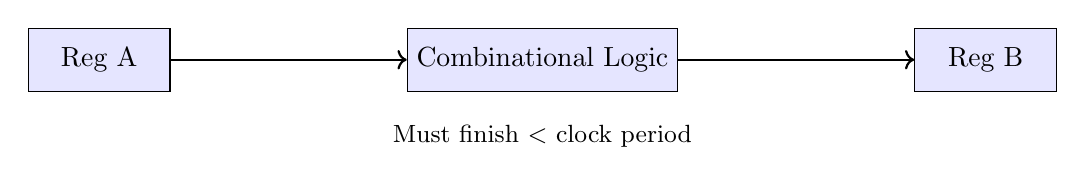
\begin{tikzpicture}[
  box/.style={draw, rectangle, minimum width=1.8cm, minimum height=0.8cm, fill=blue!10},
  arr/.style={-{Stealth}, thick}
]
\node[box] (a) {Reg A};
\node[box, right=3cm of a] (logic) {Combinational Logic};
\node[box, right=3cm of logic] (b) {Reg B};
\draw[->, thick] (a) -- (logic);
\draw[->, thick] (logic) -- (b);
\node[below=0.3cm of logic]{\small Must finish $<$ clock period};
\end{tikzpicture}
\end{center}

\vspace{0.3em}
\[
  \text{WNS} = \text{Clock Period} - \text{Critical Path Delay}
\]

\begin{itemize}
  \item WNS $> 0$ $\Rightarrow$ logic finishes in time $\Rightarrow$ \textcolor{green!60!black}{\textbf{PASS}}
  \item WNS $< 0$ $\Rightarrow$ logic misses clock edge $\Rightarrow$ \textcolor{red}{\textbf{FAIL}}
\end{itemize}

\vspace{0.3em}
\begin{alertblock}{Why parallelising does NOT improve WNS}
Parallelising reduces the number of times we traverse the critical path, not how long that path takes. Even with 500 fewer cycles, a 32 ns path still takes 32 ns to travel from register to register.
To improve WNS you must \textbf{shorten the critical path itself}.
\end{alertblock}
\end{frame}

\begin{frame}{Finding the Bottleneck with Vivado}
Vivado provides a built-in timing report listing every logic cell and its delay along the critical path:

\vspace{0.2cm}
\begin{center}
\texttt{Reports $\to$ Timing $\to$ Report Timing Summary}\\
\texttt{$\to$ Intra Clock Paths $\to$ Setup $\to$ double-click worst path}
\end{center}

\vspace{0.3em}
This revealed the critical path was \textbf{Barrett Stage 3} in the INTT scale block:

\vspace{0.2em}
\begin{center}
\small
\begin{tabular}{lll}
\toprule
\textbf{Operation} & \textbf{Implementation} & \textbf{Delay} \\
\midrule
$tq = t \times q$       & LUT/DSP chain  & $\sim$18 ns \\
$r = p - tq$             & CARRY4 chain   & $\sim$8 ns \\
if $r \geq q$: $r -= q$ & CARRY4 chain   & $\sim$6 ns \\
\midrule
\textbf{Total (one clock)} & & \textbf{32.1 ns} \\
\bottomrule
\end{tabular}
\end{center}

\vspace{0.3em}
With a 50 ns constraint: $\text{WNS} = 50 - 32.1 = \mathbf{+17.9\,\text{ns}}$
\end{frame}

\begin{frame}{DSP48 --- Dedicated Multiply Hardware}
\begin{columns}
\column{0.5\textwidth}
\textbf{LUT-based multiply:}
\begin{itemize}\small
  \item Built from thousands of general-purpose LUT gates
  \item Signal travels through every gate
  \item $\sim$31 ns for 40-bit multiply
\end{itemize}

\column{0.5\textwidth}
\textbf{DSP48-based multiply:}
\begin{itemize}\small
  \item Dedicated silicon block on the FPGA
  \item Hardwired for multiply/accumulate
  \item $\sim$3--5 ns for same operation
\end{itemize}
\end{columns}

\vspace{0.5em}
Forced in \texttt{ntt.v} using the Vivado attribute:
\begin{center}
\ttfamily\small
(* use\_dsp = "yes" *) reg [2*Q\_WIDTH-1:0] bfly\_tq;
\end{center}

\vspace{0.3em}
Applied to four registers: \texttt{bfly\_p}, \texttt{bfly\_pm}, \texttt{sc\_p}, \texttt{sc\_pm}, \texttt{bfly\_tq}, \texttt{sc\_tq}.

\vspace{0.3em}
\begin{block}{Effect}
Vivado replaces LUT multiply with DSP48 block. LUT utilisation drops; DSP utilisation rises; critical path shortens significantly.
\end{block}
\end{frame}
\end{frame}

\begin{frame}{Full Results --- All Three Versions}
\begin{center}
\small
\begin{tabular}{lcccc}
\toprule
\textbf{Metric} & \textbf{V1 (5 states)} & \textbf{V2 (8 states)} & \textbf{V3 (9 states)} & \textbf{V3 + Prefetch} \\
\midrule
States/butterfly   & 5       & 8       & 9       & 6 effective \\
Total cycles       & 266,240 & 425,984 & 479,232 & \textbf{319,488} \\
WNS                & violation & 17.9 ns & \textbf{27.5 ns} & \textbf{27.5 ns} \\
Critical path      & 60+ ns  & 32.1 ns & \textbf{22.5 ns} & \textbf{22.5 ns} \\
Max frequency      & ---     & 31 MHz  & \textbf{44 MHz}  & \textbf{44 MHz}  \\
Runtime            & ---     & 13.7 ms & 10.9 ms & \textbf{7.3 ms}  \\
\bottomrule
\end{tabular}
\end{center}

\vspace{0.3em}
\begin{columns}
\column{0.5\textwidth}
\begin{block}{Key insight}
\centering
$T_{\text{total}} = \text{Cycles} \times \text{Period}$\\
Fix timing AND reduce cycles.
\end{block}

\column{0.5\textwidth}
\begin{alertblock}{End-to-end speedup}
\centering
V2 baseline: $13.7$ ms\\
V3 + Prefetch: $7.3$ ms\\
$\approx \mathbf{1.9\times}$ overall speedup
\end{alertblock}
\end{columns}

\vspace{0.3em}
\textbf{Story:} V1 was fast but broken. V2 fixed timing but added cycles. V3 further improved timing. The prefetch recovered the cycles lost by pipelining.
\end{frame}

% ================================================================
\section{Conclusion}
% ================================================================

\begin{frame}{Summary}
\begin{enumerate}
    \item \textbf{Full BV homomorphic encryption} pipeline in pure Python
    \item \textbf{RNS decomposition} avoids large-integer arithmetic
    \item \textbf{NTT acceleration} for $O(N \log N)$ polynomial multiplication
    \item \textbf{Homomorphic hash verification} confirms computation correctness without decryption
    \item \textbf{Arithmetic circuit parser} with tree-balancing optimization
    \item \textbf{Hardware acceleration} via Verilator-compiled Verilog with transparent fallback
    \item \textbf{Cross-validation} between SW and HW via hex test vectors
\end{enumerate}

\vspace{0.5em}
\begin{block}{Key Takeaway}
Encrypted data can be computed on, verified, and accelerated in hardware ---
all without ever revealing the plaintext.
\end{block}
\end{frame}

\begin{frame}
\centering
\vspace{2cm}
{\Huge Thank You}
\vspace{1cm}

{\large Questions?}
\end{frame}

\end{document}
